% Appendix C

\chapter{Dal DEM alle curve di livello}
\label{ch:dem_to_isoipse}

In questa breve appendice vedremo come estrarre le curve di livello da un DTM (Modello digitale del terreno), attraverso QGIS.
Importiamo un DTM  all'interno dei layer di QGIS  (figura \ref{fig:QGis_DEM}).
\begin{figure}[H]
	\centering
	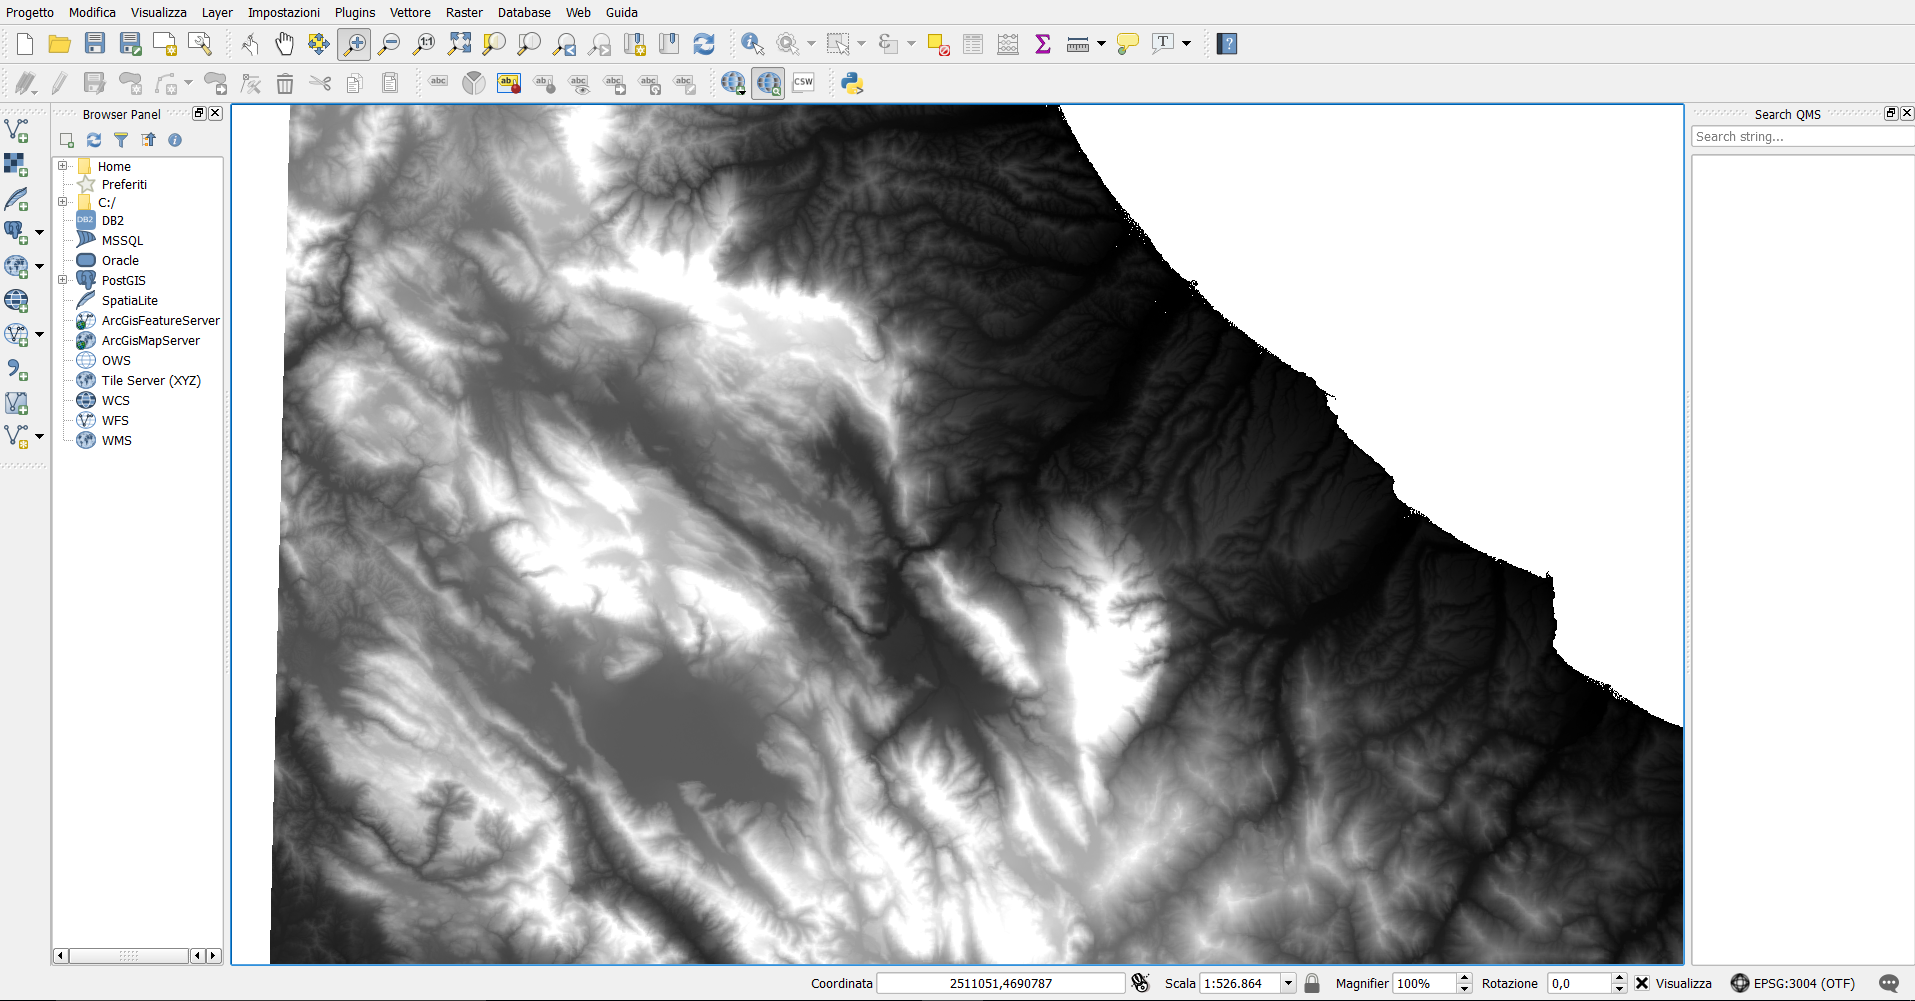
\includegraphics[width=1\textwidth]{images/QgisLivello1}
	\caption{DEM caricato all'interno di QGIS come layer}
	\label{fig:QGis_DEM}
\end{figure}
Una volta importato il layer, dal menù Raster => Estrazione => Curve di livello  (figura \ref{fig:QGis_Livello})
\begin{figure}[H]
	\centering
	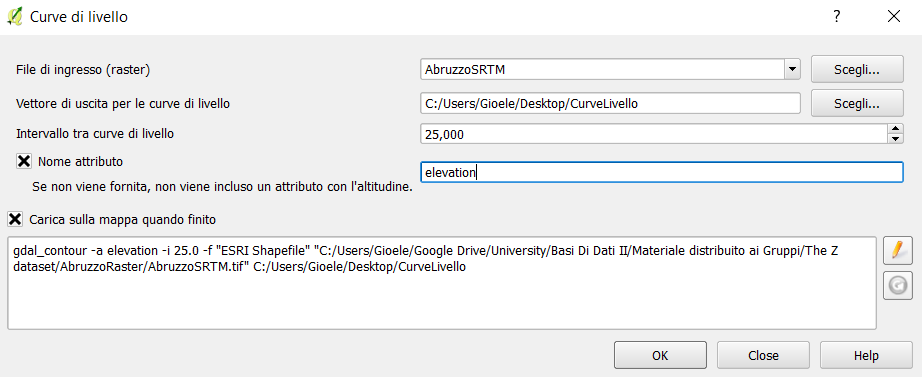
\includegraphics[width=1\textwidth]{images/CurveLivelloQGIS}
	\caption{Menù delle impostazioni per generare le curve di livello}
	\label{fig:QGis_Livello}
\end{figure}
Premendo il tasto OK verranno generate le curve di livello  (figura \ref{fig:QGis_Isoipse}).
\begin{figure}[H]
	\centering
	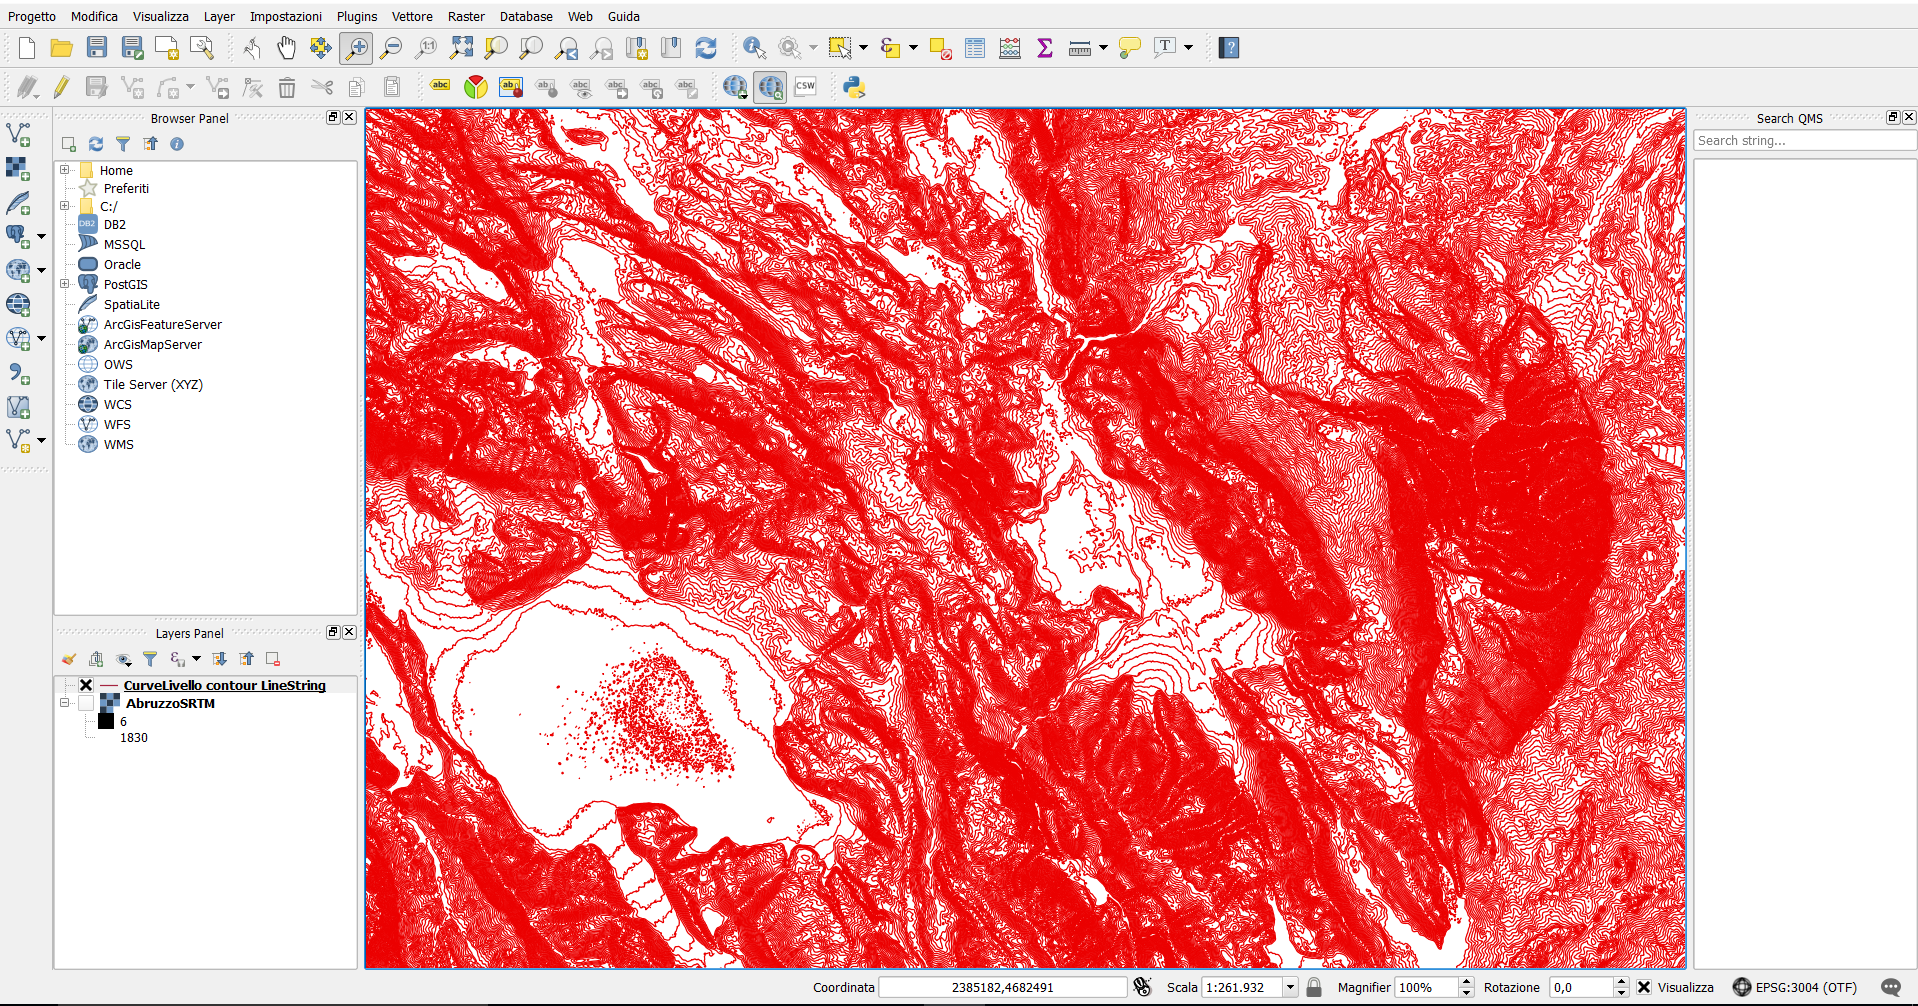
\includegraphics[width=1\textwidth]{images/IsoipseGenerate}
	\caption{Layer QGIS con le curve di livello calcolate}
	\label{fig:QGis_Isoipse}
\end{figure}
Infine intersecando le curve di livello con la $\mathcal{GEOAREA}$ dell'Abruzzo si ottengono le sole curve all'interno di essa (figura \ref{fig:QGis_Isoipse_aBruzzo}).
\begin{figure}[H]
	\centering
	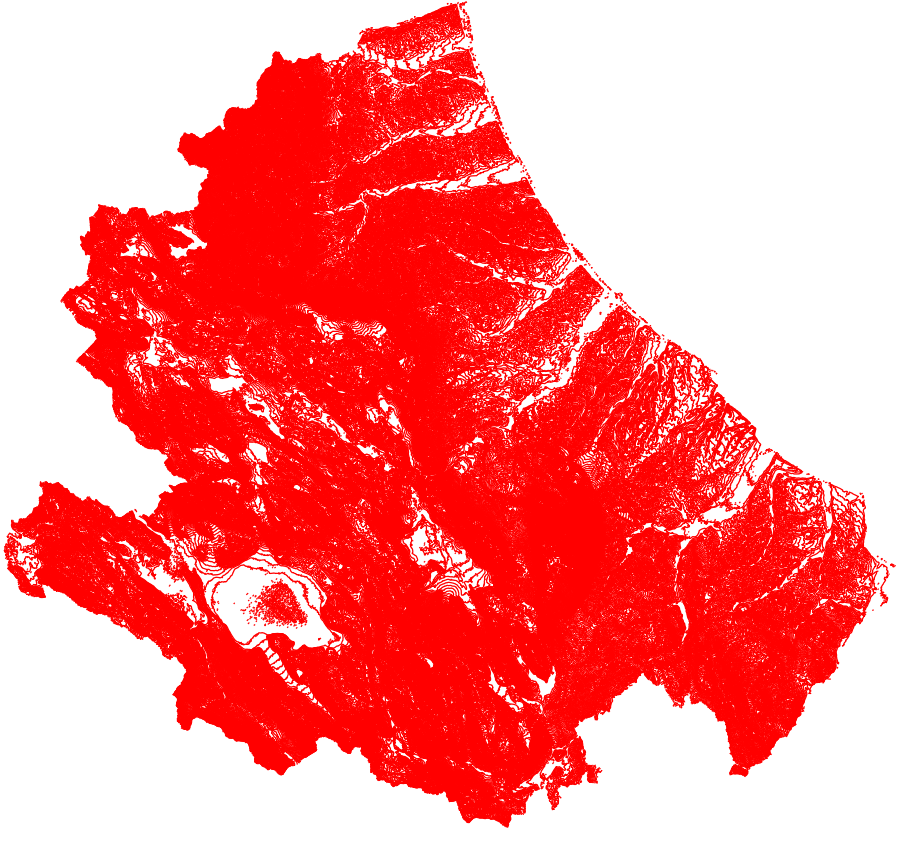
\includegraphics[width=0.7\textwidth]{images/AbruzzoIsoipse}
	\caption{Layer QGIS con le curve di livello dell'Abruzzo}
	\label{fig:QGis_Isoipse_aBruzzo}
\end{figure}